\section{АНАЛИЗ ПОДХОДОВ К РЕШЕНИЮ ПОСТАВЛЕННОЙ ЗАДАЧИ}
\label{sec:domain}
\subsection{Анализ предметной области}
В настоящий момент медицина является актуальной предметной областью, так как она играет неотъемлемую роль в жизни человека. Медицина постоянная развивается, что приводит к повышению уровня здоровья населения. Основными источниками знаний по медицине являются учебные пособия, книги, справочники, сборники статей и Интернет, однако каждый ресурс предоставляет информацию лишь о какой-то конкретной предметной области, или же рассматривает все предметные области, но поверхностно. Также ни один из источников не может достаточно гибко модернизироваться, не говоря уже о принятии единства в определении терминов. Интеллектуальная справочная система позволит собрать и структурировать всю информацию в рамках рассматриваемой предметной области, которая будет регулярно пополнятся новыми понятиями.\\
ИСС по медицине включает в себя следующие разделы:
\begin{itemize}
    \item раздел традиционной медицины;
    \item раздел нетрадиционной медицины;
    \item раздел психиатрии.\\
\end{itemize}{}


\subsection{Сравнительный анализ аналогов}
 
Рассмотрим несколько аналогов разрабатываемой ИСС по медицине, и выделим их недостатки и преимущества.
\begin{enumerate}
    \item{
    Медицинская поисковая система \cite{medpoisk}
        \newline
        Достоинства:
        \begin{itemize}
            \item{Наличие перечня клиник, болезней и способов их лечения;}
            \item{Присутствие понятийного аппарата;}
        \end{itemize}
        Недостатки:
        \begin{itemize}
            \item Предоставляемая информация не структурирована;
            \item Понятия не разделены на разделы;\\
        \end{itemize}
    На рисунке~\ref{fig:sections/medpoisk} изображен фрагмент Медицинской поисковой системы МедПоиск
    \begin{figure}[H]
    	\centering
    	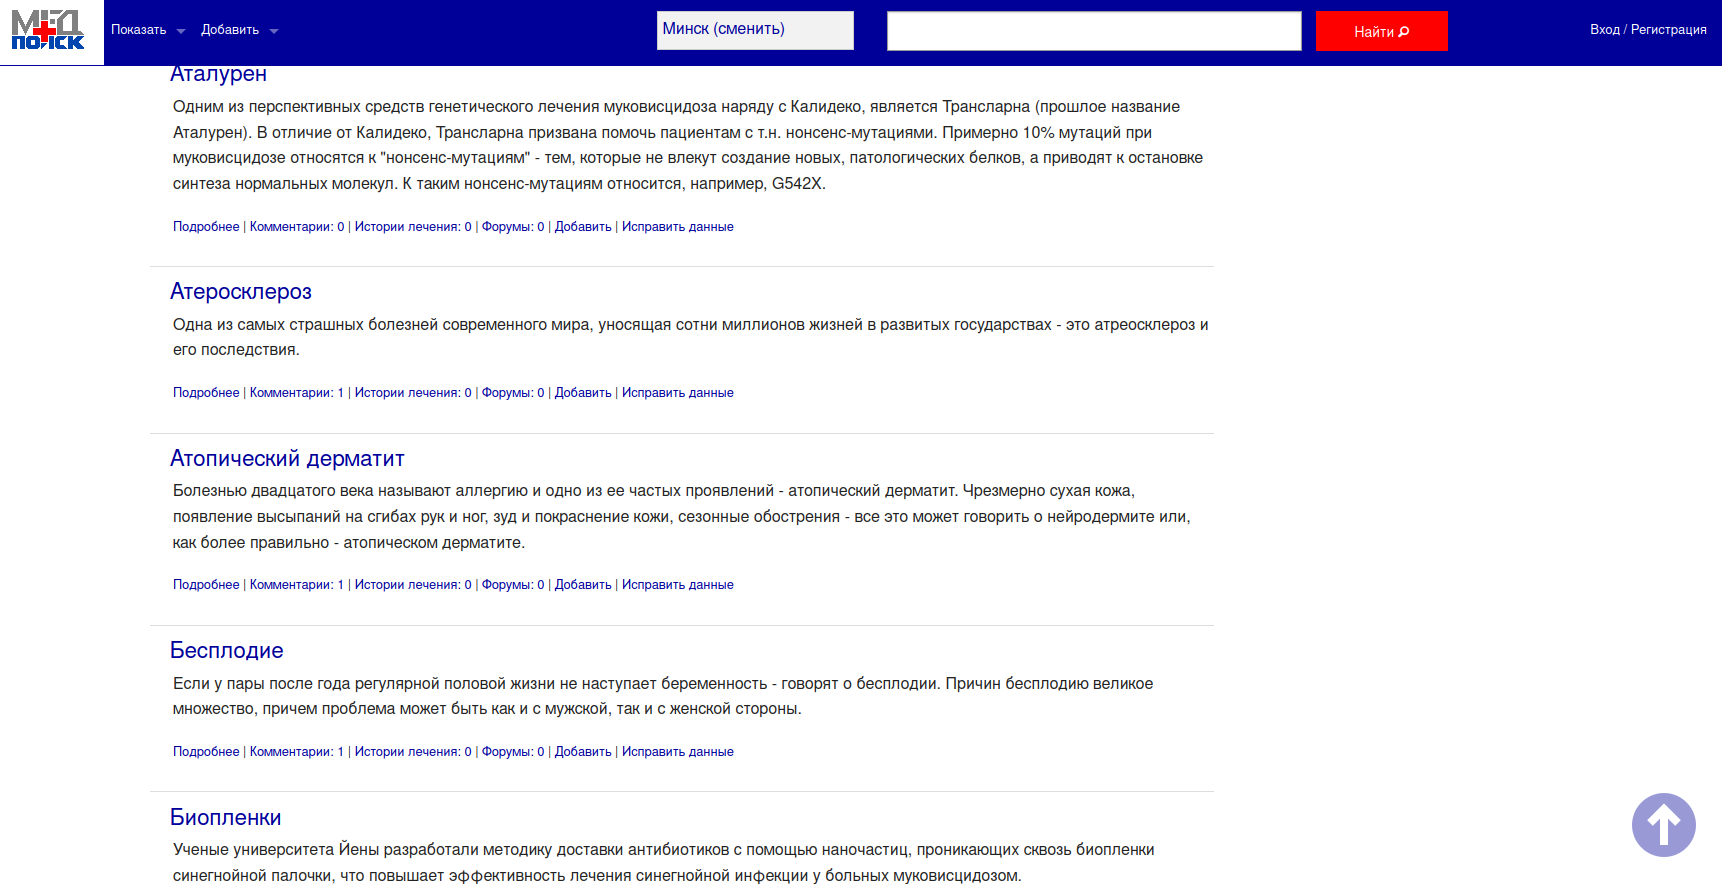
\includegraphics[width=1.0\textwidth]{sections/medpoisk}
    	\caption{Медицинская поисковая система (МедПоиск)}
     	\label{fig:sections/medpoisk}
    \end{figure}    
    }   

    \item{
       Профессиональная медицинская платформа \cite{medelement}
        \newline
        Достоинства:
        \begin{itemize}
            \item{Наличие технологии помощи в принятии клинических решений;}
            \item{Присутствие клинических терминов и способов лечения;}
        \end{itemize}
        Недостатки:
        \begin{itemize}
       	\item Узкий перечень терминов и заболеваний;
        \item {Неудобный интерфейс системы;}
        \item {Понятия не разделены на разделы;}\\
        \end{itemize}
    На рисунке~\ref{fig:sections/medelement} изображен фрагмент Профессиональной медицинской платформы MedElement
   \begin{figure}[H]
   	\centering
   	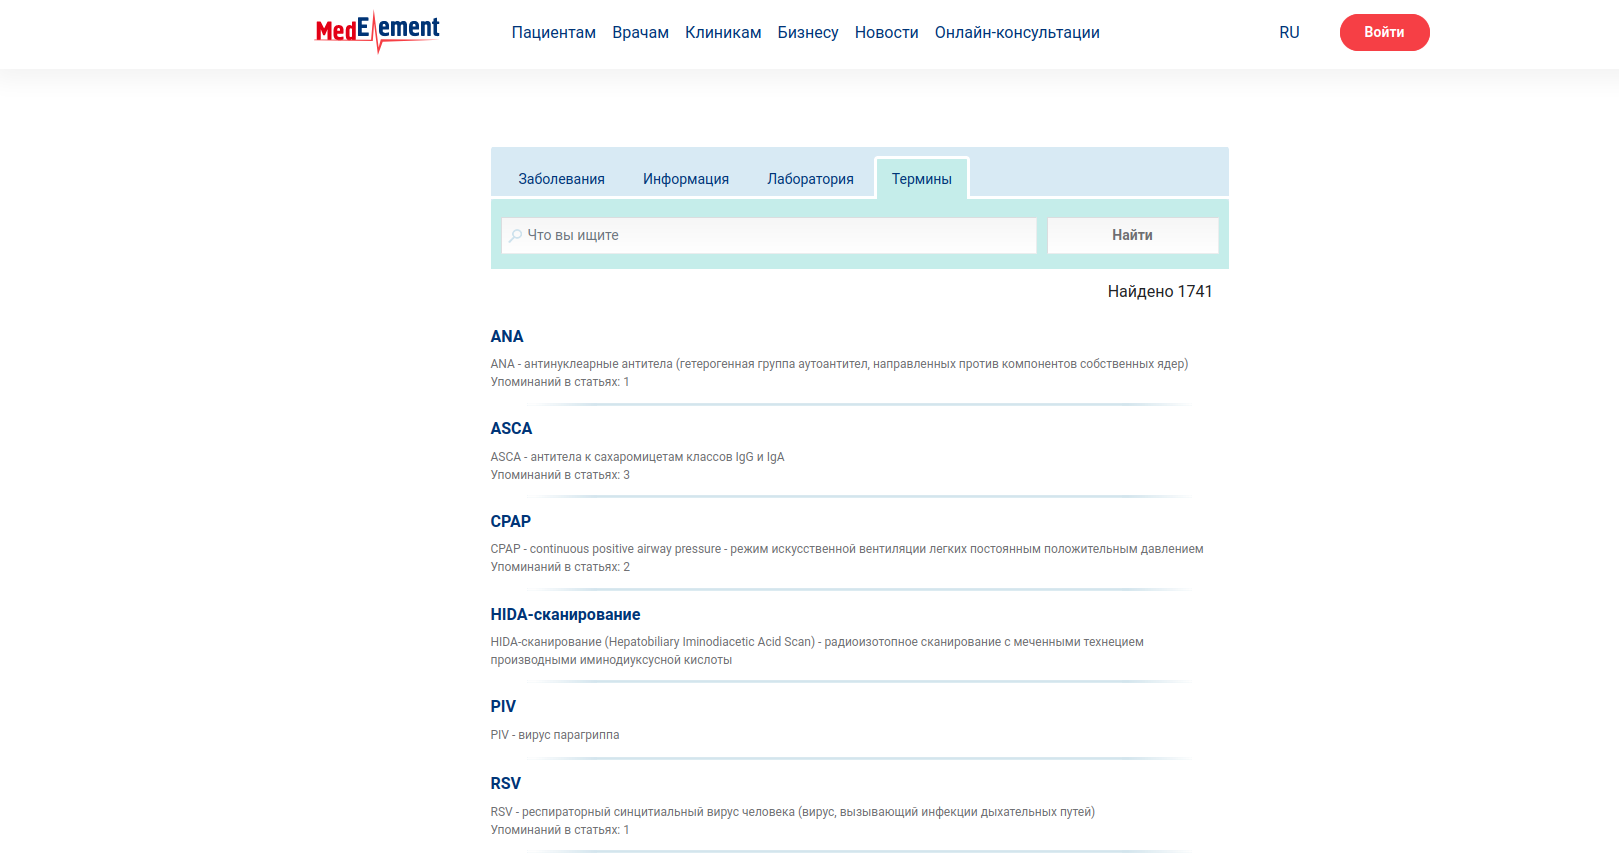
\includegraphics[width=1.0\textwidth]{sections/medelement}
   	\caption{Профессиональная медицинская платформа (MedElement)}
  	\label{fig:sections/medelement}
   \end{figure}
   
    }
\end{enumerate}

\subsection{Анализ подходов к разработке баз знаний}
Для разработки базы знаний может использоваться:
\begin{itemize}
    \item Технология OSTIS (Open Semantic Technology for Intelligent Systems);
\end{itemize}
OSTIS - открытая семантическая технология проектирования интеллектуальных систем. OSTIS позволяет представить знания в виде семантических сетей, посредством использования SC-кода (Semantic Computer Code).\cite{OSTIS} 

Основные положения:
\begin{itemize}
	\item база знаний OSTIS может описывать любой вид знаний; 
	\item решатель задач OSTIS основан на многоагентном подходе и позволяет легко комбинировать любые модели решения задач;
	\item интерфейс ostis-системы представляет собой подсистему со своей БЗ и решателем задач (также может быть описан с помощью SC-кода);
	\item использование универсального способа представления (кодирования) информации, получившего название SC-код.
\end{itemize}

Достоинства:
\begin{itemize}
	\item унифицированность представления (любая информация представляется одинаково); 
	\item удобств машинной обработки и восприятия человеком;
	\item любые знания и модели решения задач легко интегрируются в ostis-систему и её всегда можно переобучить;
	\item платформенная независимость (разработка независима от операционной системы и архитектуры компьютера, платформа может быть реализована как в программном варианте, так и в аппаратном);
	\item параллельная обработка информации;
	\item ostis-система может включать в себя компоненты, разработанные на базе OSTIS, а также объединяться с любыми другими системами и интегрировать другие компоненты через специальный протокол обмена информацией (JSON) и/или программный интерфейс (API);
	\item производительность ostis-системы не хуже традиционной системы, а иногда может оказаться лучше за счёт параллельной обработки (при переходе на семантические компьютеры производительность будет ещё выше).
\end{itemize}

Алфавит SC-кода представляет собой базовое синтаксическое разбиение множества sc-элементов на следующие виды (синтаксически задаваемые классы) \cite{OSTIS}:
\begin{itemize}
	\item sc-узел;
	\item sc-ребро;
	\item sc-дуга общего вида;
	\item sc-дуга основного вида;
\end{itemize}

SC-код позволяет представлять знания в унифицированном виде.

\begin{itemize}
	\item Semantic Web;
\end{itemize}
Семантическая паутина — надстройка над существующей Всемирной паутиной, придуманная для того, чтобы сделать размещаемую в Интернете информацию пригодной для машинной обработки. Доступная в сети информация удобна для прочтения человеком. Семантическая паутина создана для того, чтобы сделать информацию пригодной для автоматического анализа, синтеза выводов и преобразования как самих данных, так и сделанных на их основе заключений в различные представления, полезные на практике. 

Достоинства:
\begin{itemize}
	\item повышенная точность и качество информации. Semantic Web-технология позволяет улучшить точность и качество информации, позволяющие находить не только объекты, которые уже входят в некоторый список, но и новые объекты;
	\item эффективность поиска и обработки информации;
	\item расширенные возможности машинной обработки предметных областей. Semantic Web-технология позволяет создавать семантические модели для предметных областей, что открывает возможности для автоматической обработки источников данных, автоматической генерации комментариев, анализа данных;
	\item улучшенная межбазовая интеграция. Semantic Web позволяет интегрировать данные из различных источников в некой мере автоматически, что ведет к экономии времени и ресурсов для создания новых баз данных либо настройки уже существующих.
\end{itemize}

Машинная обработка возможна благодаря двум характеристикам семантической паутины:
\begin{itemize}
	\item наличие URI;
	\item использование семантических сетей и онтологий. 
\end{itemize}

URI — унифицированный идентификатор ресурса или адрес, используемый для указания ссылок на какой-либо объект (например, веб-страницу, файл или ящик электронной почты). URI используются для именования объектов. Каждый объект глобальной семантической сети имеет уникальный URI. URI однозначно называет некоторый объект. Отдельные URI создают не только для страниц, но и для объектов реального мира (людей, городов, художественных произведений и так далее), и даже для абстрактных понятий (например, «имя», «должность», «цвет»). Благодаря уникальности URI одни и те же предметы можно называть одинаково в разных местах семантической паутины. Используя URI, можно собирать информацию об одном предмете из разных мест. Рекомендуется включать в адрес URI название одного из протоколов Всемирной паутины (HTTP или HTTPS).
Описание желательно предоставлять в двух форматах:
\begin{itemize}
	\item в  формате, удобном для чтения человеком;
	\item в формате, удобном для чтения машиной.
\end{itemize}

В качестве формата, удобного для чтения машиной, используется язык RDF. Язык RDF позволяет описывать структуру семантической сети в виде графа. Каждому узлу и каждой дуге графа можно назначить отдельный URI. Утверждения, записанные на языке RDF, можно интерпретировать с помощью онтологий.

Для создания онтологий рекомендуют использовать языки RDF Schema и OWL. Онтологии создаются для получения из данных логических заключений. В основе онтологий лежат математические формализмы, называемые дескрипционными логиками.
В качестве редактора онтологий и фреймворка для построения базы знаний используется Protege.
Платформа Protege поддерживает два основных способа моделирования онтологий посредством редакторов Protege-Frames и Protege-OWL. Онтологии, построенные в Protege, могут быть экспортированы во множество форматов, включая RDF (RDF Schema), OWL и XML Schema.

Protege поддерживается значительным сообществом, состоящим из разработчиков и учёных, правительственных и корпоративных пользователей, использующих его для решения задач, связанных со знаниями, в таких разнообразных областях, как биомедицина, сбор знаний и корпоративное моделирование.

\subsection{Вывод}
На основании анализа предметной области "Медицина" можно сделать следующие выводы:

\begin{itemize}
	\item Медицина — это комплексная отрасль, включающая в себя различные области знаний и практик, направленных на сохранение и восстановление здоровья человека;
	
	\item Современная медицина основывается на научных исследованиях, технологических достижениях и практическом опыте;
	
	\item Одной из основных задач медицины является профилактика и лечение различных заболеваний, а также реабилитация пациентов после их выздоровления;
	
	\item В медицине широко применяются различные методы диагностики и лечения, включающие в себя медикаментозную терапию, хирургические вмешательства, физиотерапию, психотерапию и т.д.
\end{itemize}{}
Анализ данных систем-аналогов приводит нас к выводу о том, что медицина - сфера , которая постоянно меняется со временем, в связи с чем, все источники инфомации по ней постоянно устаревают, или же теряют свою актуальность, поэтому проектируемая система должна иметь следующие качества:
\begin{itemize}
	\item {база знаний, достаточная для удовлетворения запросов пользователя и которая будет постоянно пополняться и обновляться;}
	
	\item{возможность производить семантический разбор исходного кода программы;}
	
	\item{пользовательский интерфейс, упрощающий пользователю работу с системой.}
\end{itemize}
Анализ подходов к разработке баз знаний показывает, что существует множество методов для создания и поддержки эффективных баз знаний. Большинство из них включает в себя процессы сбора, хранения, классификации и анализа данных, а также определение правил интеллектуальной обработки этих данных.

Однако универсальным подходом, который мог бы обеспечить разработку эффективных баз знаний, не существует. Это связано не только с техническими аспектами, но и с тем, что различные объекты и данные могут иметь разную степень сложности и свойства. 

Одним из важных аспектов является поддержка базы знаний. Разработчики должны обеспечивать постоянное обновление базы знаний, чтобы она оставалась актуальной и эффективной. 

Таким образом, для эффективной разработки баз знаний необходимо тщательно выбирать подходы и методы, которые будут правильно соответствовать типу приложений или задач, а также обеспечивать постоянную поддержку и обновление базы знаний.
\section{ПРОЕКТИРОВАНИЕ БАЗЫ ЗНАНИЙ}
\subsection{Архитектура базы знаний по медицине}
Целями создания ИСС по медицине является структурирование знаний по медицине ,которые в будущем смогут облегчить предоставление пользователю точной и своевременной информации о здоровье, болезнях и лечении болезней. Также, она  может быть полезна в обучении студентов медицинских учебных заведений и повышения квалификации врачей.

Планируется создание системы,которая сможет позволить совершить запрос пользователю по интересующему его вопросу и получить название термина на русском, английском и латинском языках, что будет полезно, как врачам так и студентам медицинских вузов, поскольку в медицинских учреждениях врачи, используя латинские термины и выписывают рецепты, таким образом, больше не будет необходимости в том, чтобы искать названия терминов в словарях или других ресурсах, вся важная и нужная информация будет локализована в одном месте, это облегчит обучение и сэкономит время.

Помимо этого система будет снабжена различными информационными иллюстрациями по темам, с помощью которых пользователи смогут визуализировать представленную по запросу информацию, что способствует лучшему пониманию и усвоению новой информации. 

Для терминов заболеваний, планируется создание симптоматики, которая будет представлена в виде нумерованного списка. 

Планируется создание структурированной и достаточно полной базы с всей необходимой информацией в области медицины, которая будет локализована в одном месте, что является значительным преимуществом в эксплуатации данной базы.
Поскольку в медицине огромное множество областей и разделов, мы не сможем охватить их все в рамках только лишь нашего курсового проекта, поэтому данная интеллектуальная справочная система будет дорабатываться и пополняться в будущем другими студентами. 
\subsection{Структура базы знаний по медицины}
База знаний по медицине состоит из одного основного раздела ПрО Медицины, который, в свою очередь, включает 2 раздела в каждом из которых есть соответствующие подразделы. 
\begin{enumerate}
	\item ПрО традиционной медицины,состоит из 5 разделов:
	\begin{enumerate}
		\item ПрО дерматологии
		ПрО дерматологии включает 4 раздела:	
		\begin{itemize}
			\item ПрО дермато-венерологии
			\item ПрО дермато-онкологии
			\item ПрО трихологии 
			\item ПрО косметологии\\
		\end{itemize}	
		\item ПрО психиатрии
		ПрО психиатрии состоит из 4 разделов:	
		\begin{itemize}
			\item ПрО детской психиатрии
			\item ПрО психиатрии позднего возраста
			\item ПрО военной психиатрии 
			\item ПрО судебной психиатрии\\
		\end{itemize}	
		\item ПрО педиатрии
		ПрО педиатрии состоит из 2 разделов:	
		\begin{itemize}
			\item ПрО профилактической педиатрии
			\item ПрО клинической педиатрии\\
		\end{itemize}	
		\item ПрО офтальмологии
		ПрО офтальмологии подразделяется на 3 раздела:	
		\begin{itemize}
			\item ПрО анатомии глаза человека
			\item ПрО рефракции глаза
			\item ПрО болезней глаза и его придатков\\
		\end{itemize}	
		\item ПрО кардиологии состоит из 5 разделов:
		\begin{itemize}
			\item ПрО клинической электрофизиологии сердца
			\item ПрО сердечной недостаточности и трансплантационной кардиологии
			\item ПрО ядерной кардиологии
			\item ПрО врожденных пороков сердца у взрослых
			\item ПрО эхокардиографии\\
		\end{itemize}
	\end{enumerate}
	\item ПрО нетрадиционной медицины, состоит из 3 разделов:
	\begin{enumerate}
		\item ПрО гомеопатии
		\item ПрО натуропатии
		\item ПрО акупунктуры (иглоукалывания)\\
		\end{enumerate}
\end{enumerate}
На рисунке~\ref{fig:sections/map} изображена структура БЗ по медицине в виде mind map диаграммы.
\begin{figure}[H]
	\centering
	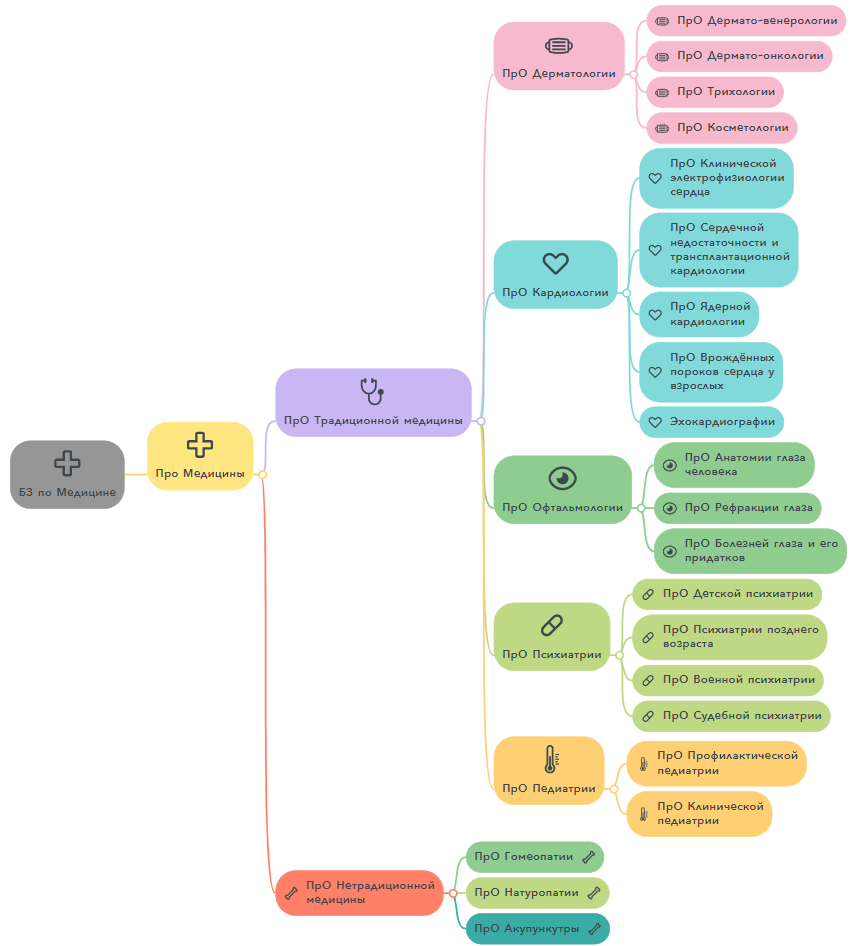
\includegraphics[width=0.95\textwidth]{sections/map.jpeg}
	\caption{Структура БЗ по медицине}
	\label{fig:sections/map}
\end{figure}
\subsection{Характеристика пользователей системы}
Категории пользователей, которыми может быть использована данная система:
\begin{itemize}
	\item Студенты медики;
	\item Преподаватели в медучреждениях;
	\item Медики;
	\item Люди, интересующиеся медициной.
\end{itemize}
Сценарии использования БЗ пользователями отображены на рисунке~\ref{fig:sections/users}.
\begin{figure}[H]
	\centering
	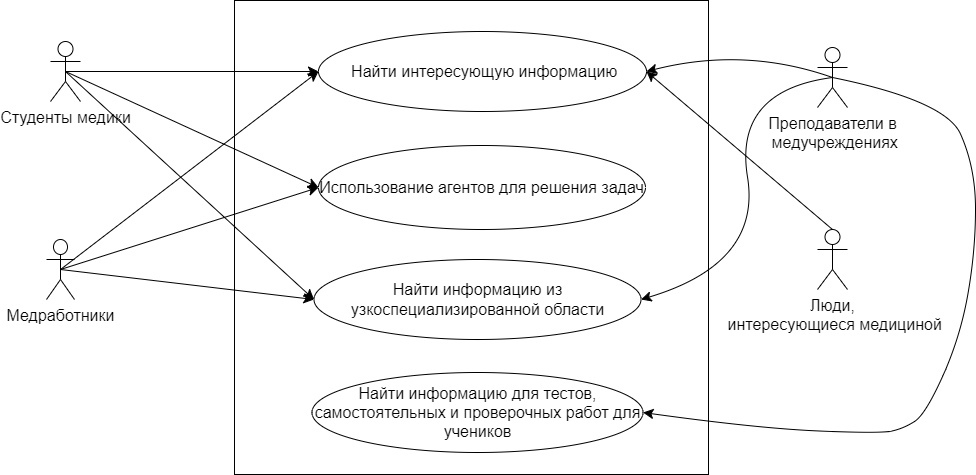
\includegraphics[width=1.0\textwidth]{sections/users.jpeg}
	\caption{Сценарии использования}
	\label{fig:sections/users}
\end{figure}

\subsection{Спецификация Предметной области  медицины}
Данная предметная область состоит из следующих разделов:
\begin{enumerate}
	\item ПрО традиционной медицины
	\item ПрО нетрадиционной медицины\\
\end{enumerate}

В свою очередь, данные предметные области также декомпозируются на разделы.

ПрО медицины содержит в себе следующие понятия, необходимые для других разделов данной предметной области:
\begin{itemize}
	\item медицина
	\item здоровье
	\item организм 
	\item орган
	\item заболевание*
	\item медикамент
	\item рецепт
	\item врач
	\item пациент 
	\item инвалидность*
	\item диагноз
	\item реабилитация*
	\item диагностика*
	\item профилактика*
	\item обследование* 
	\item симптом*
	\item синдром*
	\item лечение* 
	\item действующее вещество*
	\item строение*
	\item местоположение*
	\item профилактика*
	\item кровь
	\item эритроциты
	\item лейкоциты
	\item тромбоциты
	\item моча
	\item анализ 
	\item иммунная система
	\item хромосома 
	\item ткань
	\item антитело\\
\end{itemize}

\subsection{Спецификация элементов предметной области медицины}
Про медицины содержит:
\begin{enumerate}
	\item максимальный класс объектов исследования: медицина
	\item немаксимальный класс объектов исследования: 
	\begin{itemize}
		\item традиционная медицина
		\item нетрадиционная медицина\\
	\end{itemize}
	
	\item отношение "заболевание" содержит домены:
	\begin{itemize}
		\item первый домен: симптом*
		\item второй домен: диагноз\\
	\end{itemize}
	
	\item отношение "инвалидность" содержит домены:
	\begin{itemize}
		\item первый домен: пациент
		\item второй домен: диагноз\\
	\end{itemize}
	
	\item отношение "реабилитация" содержит домены:
	\begin{itemize}
		\item первый домен: пациент
		\item второй домен: здоровье\\
	\end{itemize}
	
	\item отношение "диагностика" содержит домены:
	\begin{itemize}
		\item первый домен: заболевание*
		\item второй домен: диагноз\\
	\end{itemize}
	
	\item отношение "профилактика" содержит домены:
	\begin{itemize}
		\item первый домен: пациент
		\item второй домен: здоровье\\
	\end{itemize}
	
	\item отношение "обследование" содержит домены:
	\begin{itemize}
		\item первый домен: заболевание*
		\item второй домен: диагностика*\\
	\end{itemize}
	
	\item отношение "симптом" содержит домены:
	\begin{itemize}
		\item первый домен: заболевание*
		\item второй домен: диагноз\\
	\end{itemize}
	
	\item отношение "синдром" содержит домены:
	\begin{itemize}
		\item первый домен: заболевание*
		\item второй домен: симптом*\\
	\end{itemize}
	
	\item отношение "лечение" содержит домены:
	\begin{itemize}
		\item первый домен: заболевание*
		\item второй домен: медикамент\\
	\end{itemize}
	
	\item отношение "действующее вещество" содержит домены:
	\begin{itemize}
		\item первый домен: вещество
		\item второй домен: медикамент\\
	\end{itemize}
	
	\item отношение "строение" содержит домены:
	\begin{itemize}
		\item первый домен: орган
		\item второй домен: организм\\
	\end{itemize}
	
	\item отношение "местоположение" содержит домены:
	\begin{itemize}
		\item первый домен: орган
		\item второй домен: организм\\
	\end{itemize}
	
\end{enumerate}

\subsection{Спецификация Предметной области традиционной медицины}
Данная предметная область состоит из следующих разделов:
\begin{enumerate}
	\item ПрО дерматологии
	\item ПрО кардиологии
	\item ПрО офтальмологии 
	\item ПрО психиатрии
	\item ПрО педиатрии\\
\end{enumerate}

В свою очередь, данные предметные области также декомпозируются на разделы.

Каждый из этих разделов содержит перечень определенных формализованных понятий.

ПрО традиционной медицины содержит понятие:
\begin{itemize}
	\item традиционная медицина\\
\end{itemize}

\subsection{Спецификация элементов предметной области традиционной медицины}
Про традиционной медицины содержит:
\begin{enumerate}
	\item максимальный класс объектов исследования: традиционная медицина
	\item немаксимальный класс объектов исследования: \begin{itemize}
		\item психиатрия
		\item офтальмология
		\item дерматология 
		\item кардиология   
		\item педиатрия\\
	\end{itemize}
\end{enumerate}

\subsection{Спецификация предметной области нетрадиционной медицины}
Данная предметная область состоит из следующих разделов:
\begin{enumerate}
\item ПрО гомеопатии
\begin{itemize}
	\item гомеопатия Ганемана (классическая гомеопатия)
	\item гомотоксикология Ганс-Генриха Рекевега
	\item гомеопатия Эпштейна
\end{itemize}

ПрО гомеопатии содержит следующие понятия:
\begin{itemize}
	\item гомеопатия 
	\item гомеопат 
	\item гомеопатический препарат*\\
\end{itemize}

\item ПрО натуропатии
\begin{itemize}
	\item аромотерапия
	\item аэрофитотерапия
	\item апитерапия 
	\item аэроинтотерапия
	\item галотерапия
	\item гелиотерапия
	\item гидротерапия
	\item гирудотерапия
	\item дендротерапия
	\item литотерапия
	\item музыкотерапия 
	\item талассотерапия
	\item лечебное голодание
	\item фитотерапия
	\item флоротерапия
	\item фунготерапия
	\item энотерапия\\
\end{itemize}

ПрО натуропатии содержит следующие понятия:
\begin{itemize}
	\item натуропатия 
	\item натуропат\\
\end{itemize}

В свою очередь, каждые из разделов имеет такие понятия как:
\begin{itemize}
	\item аромотерапия
	\item аэрофитотерапия
	\item апитерапия 
	\item аэроинтотерапия
	\item галотерапия
	\item гелиотерапия
	\item гидротерапия
	\item гирудотерапия
	\item дендротерапия
	\item литотерапия
	\item музыкотерапия 
	\item талассотерапия
	\item лечебное голодание
	\item фитотерапия
	\item флоротерапия
	\item фунготерапия
	\item энотерапия\\
\end{itemize}

\item ПрО акупунктуры

ПрО акупунктуры содержит следующие понятия:
\begin{itemize}
	\item акупунктура 
	\item игла медицинская
	\item акупунктурная точка\\
\end{itemize}
\end{enumerate} 

ПрО нетрадиционной медицины содержит понятие:
\begin{itemize}
	\item нетрадиционная медицина\\
\end{itemize}

\subsection{Спецификация элементов предметной области нетрадиционной медицины}
Про нетрадиционной медицины содержит:
\begin{enumerate}
	\item максимальный класс объектов исследования: нетрадиционная медицина
	\item немаксимальный класс объектов исследования: \begin{itemize}
		\item гомеопатия 
		\item натуропатия
		\item акупунктура\\
	\end{itemize}
\end{enumerate}

\subsection{Спецификация предметной области психиатрии}
Про психиатрии включает в себя 4 раздела:
\begin{enumerate}
	\item ПрО детской психиатрии
	\item ПрО психиатрии позднего возраста
	\item ПрО военной психиатрии 
	\item ПрО судебной психиатрии\\
\end{enumerate}

ПрО психиатрии содержит в себе следующие понятия, необходимые для других разделов данной предметной области:
\begin{itemize}
	\item психиатрия
	\item психика
	\item психиатр 
	\item личность
	\item психическое расстройство
	\item психотропное вещество
	\item поведение
	\item эмоции
	\item память 
	\item мышление
	\item сознание
	\item галлюцинации
	\item бред
	\item возбуждение
	\item тревога 
	\item расстройство настроения
	\item расстройство личности
	\item невротическое расстройство
	\item поведенческий синдром
	\item шизоактивное расстройство\\
\end{itemize}

\subsection{Спецификация элементов предметной области психиатрии}
Про психиатрии содержит:
\begin{enumerate}
	\item максимальный класс объектов исследования: психиатрия
	\item немаксимальный класс объектов исследования: \begin{itemize}
		\item детская психиатрия
		\item психиатрия позднего возраста
		\item военная психиатрия 
		\item судебная психиатрия\\
	\end{itemize}
\end{enumerate}


\subsection{Вывод}
В результате проектирования базы знаний по медицине и, в частности,
ПрО медицины, ПрО традиционной медицины, ПрО нетрадиционной медицины и ПрО психиатрии была создана эффективная система хранения и управления медицинскими знаниями. База знаний содержит
информацию о строении определённых органов и систем органов человека, различных заболеваниях, их симптоматику, а также перевод всех терминов на латинский язык.

Важным элементом проектирования базы знаний является возможность ее дальнейшего развития и модификации.

База знаний может быть расширена новыми сведениями о заболеваниях, методах лечения и препаратах, а также может быть адаптирована под различные медицинские специальности.


\section{РЕАЛИЗАЦИЯ БАЗЫ ЗНАНИЙ ПО МЕДИЦИНЕ}
\subsection{Средства, используемые при реализации}
Для реализации ПрО медицины была использована технология OSTIS. Для представления знаний в интеллектуальных системах используется базовый язык – SC-код. SC-код-- способ универсального смыслового представления информации в памяти компьютерных систем. Он основан на теории графов, теории множеств, что обеспечивает универсальность и унифицированность представления информации, удобство машинной обработки и восприятия человеком. С помощью SC-кода можно описывать базы знаний, решатели задач и интерфейс интеллектуальной системы. SC-code является абстрактным языком, но его можно визуализировать в различных формах.\cite{OSTIS}

Формы внешнего представления SC-кода
\begin{itemize}
	\item {SCs (текстовый линейный)}
	\item {SCn (гипертекстовый)}
	\item {SCg (графический)}
\end{itemize}
 

Для описания понятий использовался подъязык SC-кода - SCs.
SCs-код - линейный вариант представления SC-кода. SCs-код представляет собой множество sc.s-текстов, каждый из которых состоит из sc.s-предложений, разделенных друг от друга двойной точкой с запятой (разделителем sc.s-предложений). При этом sc.s-предложение представляет собой последовательность sc-идентификаторов, являющихся именами описываемых сущностей и разделяемых между собой различными sc.s-разделителями и sc.s-ограничителями.

Для упрощения процесса разработки исходных текстов баз знаний с использованием SCs-кода вводятся два алфавита символов. Базовый алфавит символов, используемых в sc.s-коннекторах включает только символы, имеющиеся на стандартной современной клавиатуре. Таким образом, для разработки исходных текстов баз знаний, использующих только базовый алфавит символов, используемых в sc.s-коннекторах достаточно обычного текстового редактора. Расширенный алфавит символов, используемых в sc.s-коннекторах включает также дополнительные символы, которые позволяют сделать sc.s-тексты более читабельными и наглядными. Для визуализации и разработки таких sc.s-текстов требуется наличие специальных средств.

Пример формализации понятия с помощью SCs-кода ~\ref{fig:sections/SCs}.
\begin{figure}[H]
	\centering
	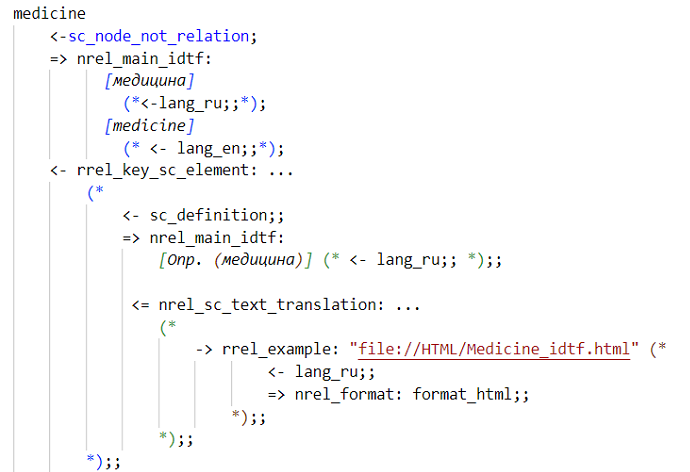
\includegraphics[width=0.7\textwidth]{sections/scs_medicine.png}
	\caption{SCs-код}
	\label{fig:sections/SCs}
\end{figure}

Пример формализации понятия с помощью языка разметки гипертекста HTML~\ref{fig:sections/HTML}.
\begin{figure}[H]
	\centering
	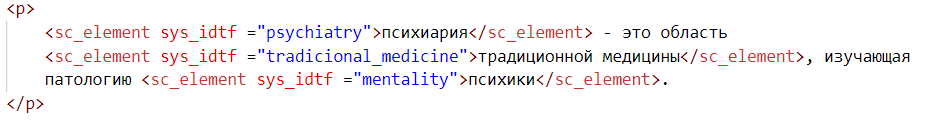
\includegraphics[width=1.0\textwidth]{sections/html_psychiatry.png}
	\caption{HTML}
	\label{fig:sections/HTML}
\end{figure}

\subsection{Примеры описания фрагментов базы знаний}
Фрагмент базы знаний, отображающий предметную область психиатрия$,$ представлен на рисунке~\ref{fig:sections/subject_domain_of_psychiatry}.
\begin{figure}[H]
	\centering
	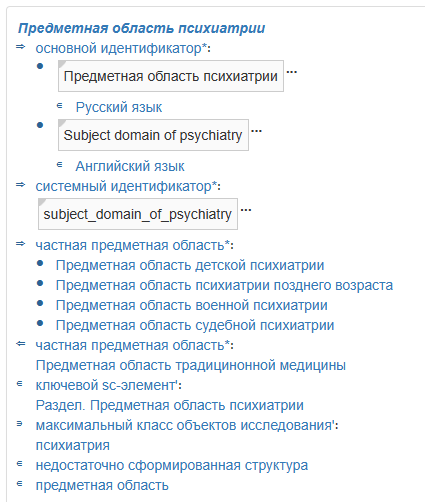
\includegraphics[width=0.55\textwidth]{sections/subject_domain_of_psychiatry.png}
	\caption{Предметная область психиатрии}
	\label{fig:sections/subject_domain_of_psychiatry}
\end{figure}

Фрагмент базы знаний, отображающий раздел ПрО психиатрии$,$ представлен на рисунке
~\ref{fig:sections/section_of_psychiatry}.
\begin{figure}[H]
	\centering
	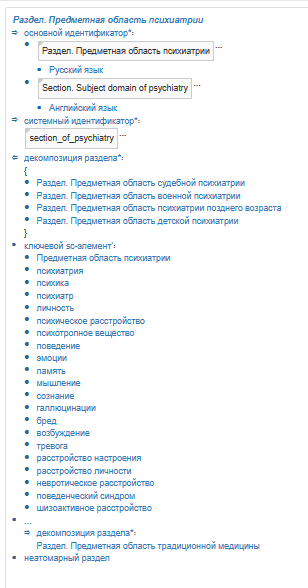
\includegraphics[width=0.5\textwidth]{sections/section_of_psychiatry.png}
	\caption{Раздел. Предметная область психиатрии}
	\label{fig:sections/section_of_psychiatry}
\end{figure}

Фрагмент базы знаний, отображающий понятие "Психиатрия"$,$ представлен на рисунке
~\ref{fig:sections/concept_psychiatry}.
\begin{figure}[H]
	\centering
	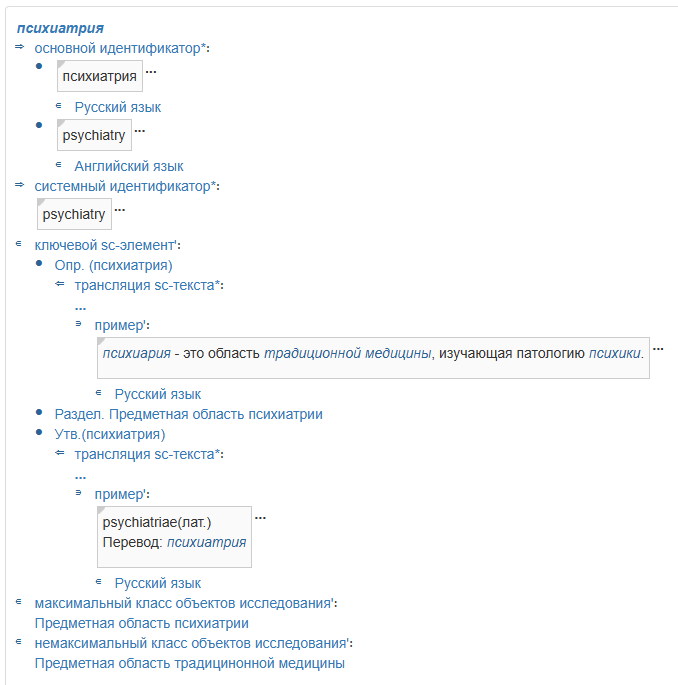
\includegraphics[width=1.0\textwidth]{sections/concept_psychiatry.png}
	\caption{Понятие "Психиатрия"}
	\label{fig:sections/concept_psychiatry}
\end{figure}

Фрагмент базы знаний, отображающий  раздел Про медицины$,$ представлен на рисунке
~\ref{fig:sections/section_of_medicine}.
\begin{figure}[H]
	\centering
	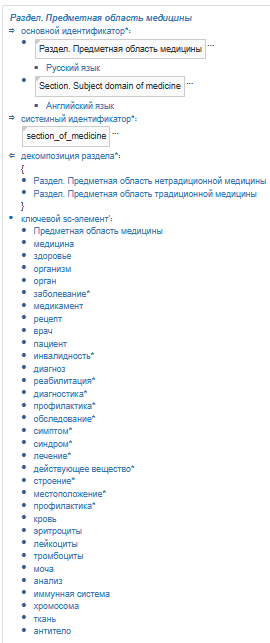
\includegraphics[width=0.5\textwidth]{sections/section_of_medicine.png}
	\caption{Раздел. Предметная область медицины}
	\label{fig:sections/section_of_medicine}
\end{figure}
Фрагмент базы знаний, отображающий предметную область медицины$,$ представлен на рисунке
~\ref{fig:sections/subject_domain_of_medicine}.
\begin{figure}[H]
	\centering
	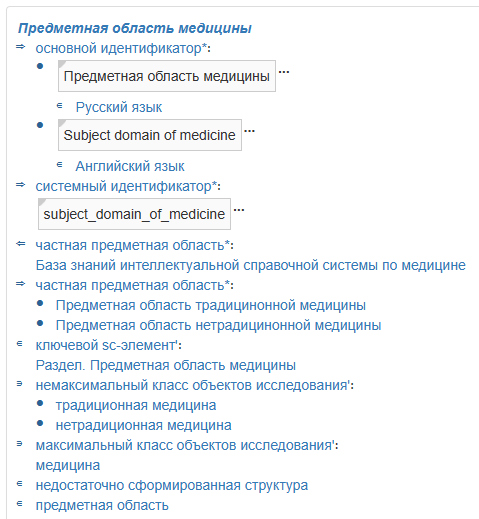
\includegraphics[width=0.55\textwidth]{sections/subject_domain_of_medicine.png}
	\caption{Предметная область медицины}
	\label{fig:sections/subject_domain_of_medicine}
\end{figure}

Фрагмент базы знаний, отображающий  раздел Про традиционной медицины$,$ представлен на рисунке
~\ref{fig:sections/section_of_traditional_medicine}.
\begin{figure}[H]
	\centering
	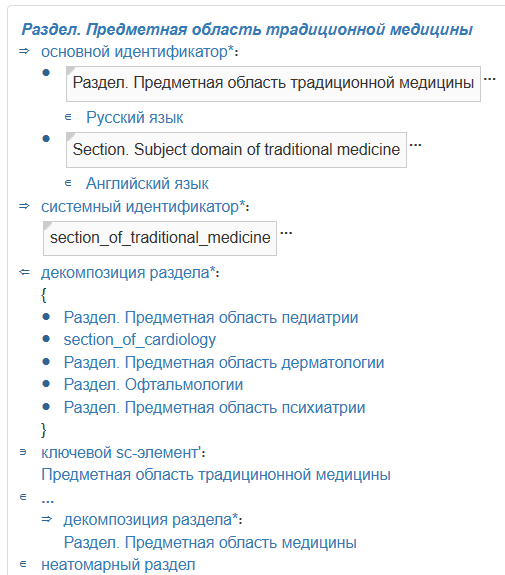
\includegraphics[width=0.7\textwidth]{sections/section_of_traditional_medicine.png}
	\caption{Раздел. Предметная область традиционной медицины}
	\label{fig:sections/section_of_traditional_medicine}
\end{figure}
Фрагмент базы знаний, отображающий предметную область традиционной медицины$,$ представлен на рисунке
~\ref{fig:sections/subject_domain_of_traditional_medicine}.
\begin{figure}[H]
	\centering
	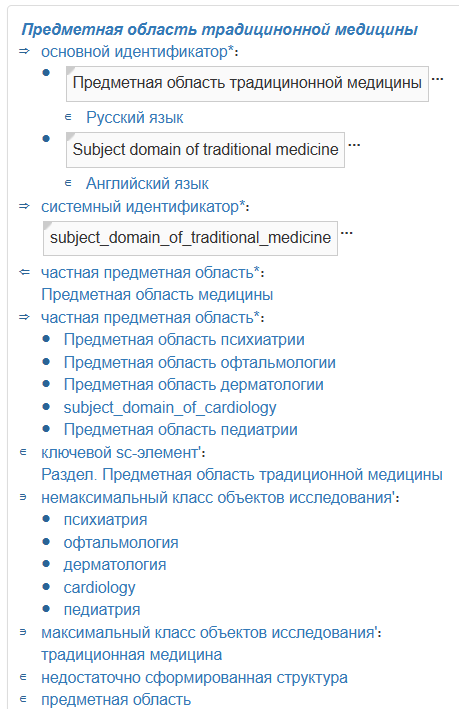
\includegraphics[width=0.55\textwidth]{sections/subject_domain_of_traditional_medicine.png}
	\caption{Предметная область традиционной медицины}
	\label{fig:sections/subject_domain_of_traditional_medicine}
\end{figure}

Фрагмент базы знаний, отображающий  раздел ПрО нетрадиционной медицины$,$ представлен на рисунке ~\ref{fig:sections/section_of_alternative_medicine}.
\begin{figure}[H]
	\centering
	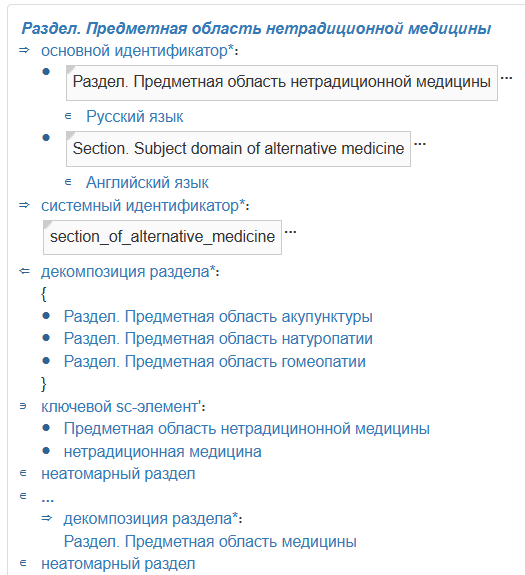
\includegraphics[width=0.55\textwidth]{sections/section_of_alternative_medicine.png}
	\caption{Раздел. Предметная область нетрадиционной медицины}
	\label{fig:sections/section_of_alternative_medicine}
\end{figure}

Фрагмент базы знаний, отображающий предметную область нетрадиционной медицины$,$ представлен на рисунке
~\ref{fig:sections/subject_domain_of_alternative_medicine}.
\begin{figure}[H]
	\centering
	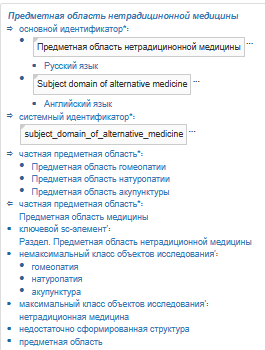
\includegraphics[width=0.5\textwidth]{sections/subject_domain_of_alternative_medicine.png}
	\caption{Предметная область нетрадиционной медицины}
	\label{fig:sections/subject_domain_of_alternative_medicine}
\end{figure}

Фрагмент базы знаний, отображающий  понятие "Медицина" \cite{bme}$,$ представлен на рисунке
~\ref{fig:sections/concept_medicine}.
\begin{figure}[H]
	\centering
	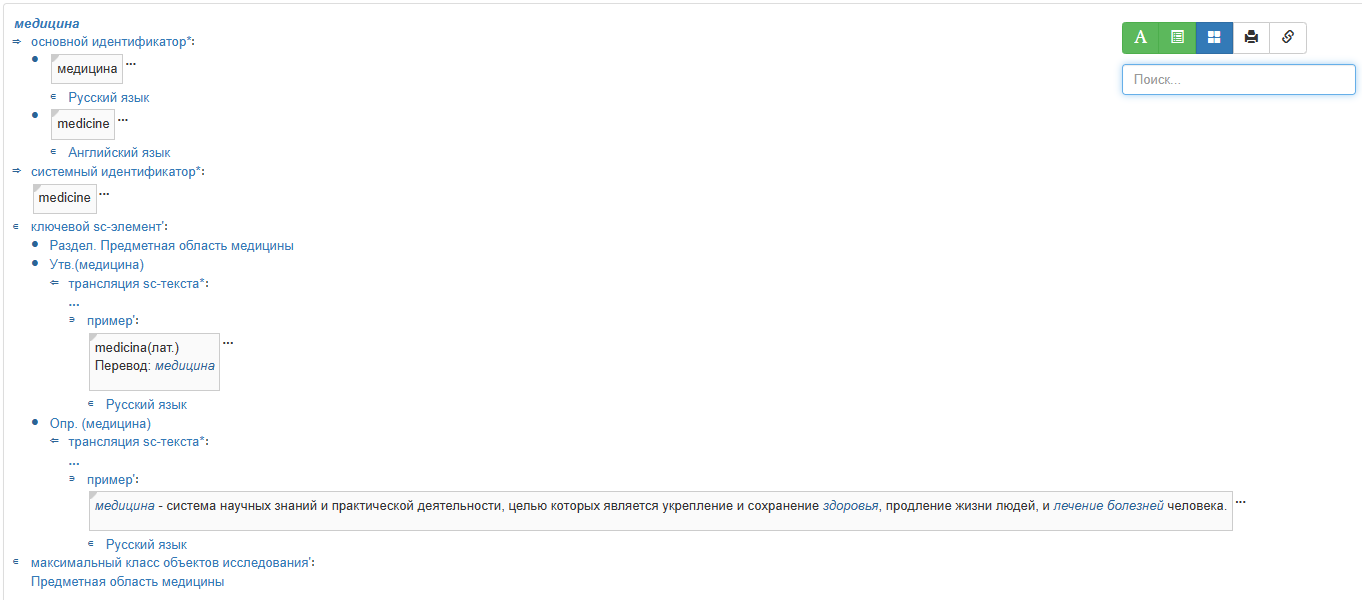
\includegraphics[width=1.0\textwidth]{sections/concept_medicine.png}
	\caption{Понятие "Медицина"}
	\label{fig:sections/concept_medicine}
\end{figure}

Фрагмент базы знаний, отображающий  понятие "Эритроциты" \cite{bme}$,$ представлен на рисунке
~\ref{fig:sections/red_blood_cells}.
\begin{figure}[H]
	\centering
	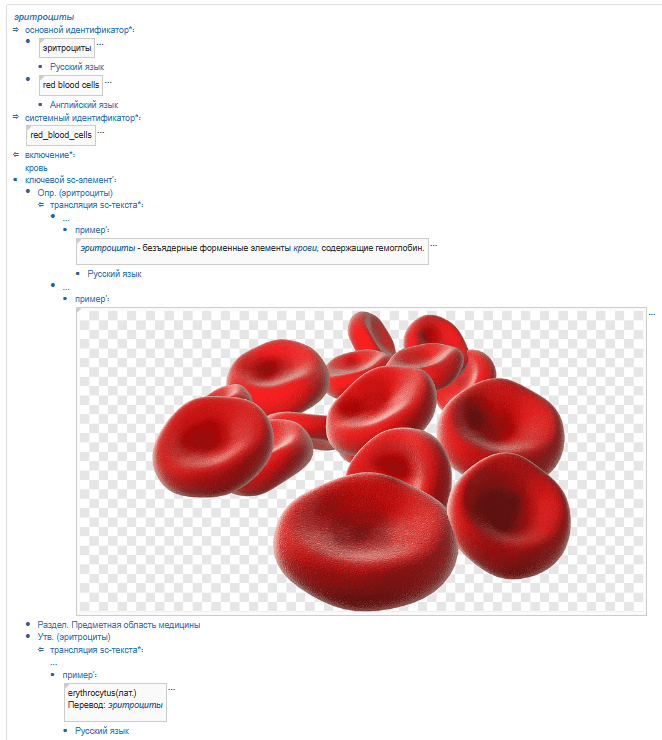
\includegraphics[width=0.7\textwidth]{sections/red_blood_cells.png}
	\caption{Понятие "Эритроциты"}
	\label{fig:sections/red_blood_cells}
\end{figure}


Фрагмент базы знаний, отображающий  понятие "Доктор" \cite{bme}$,$ представлен на рисунке
~\ref{fig:sections/concept_doctor}.
\begin{figure}[H]
	\centering
	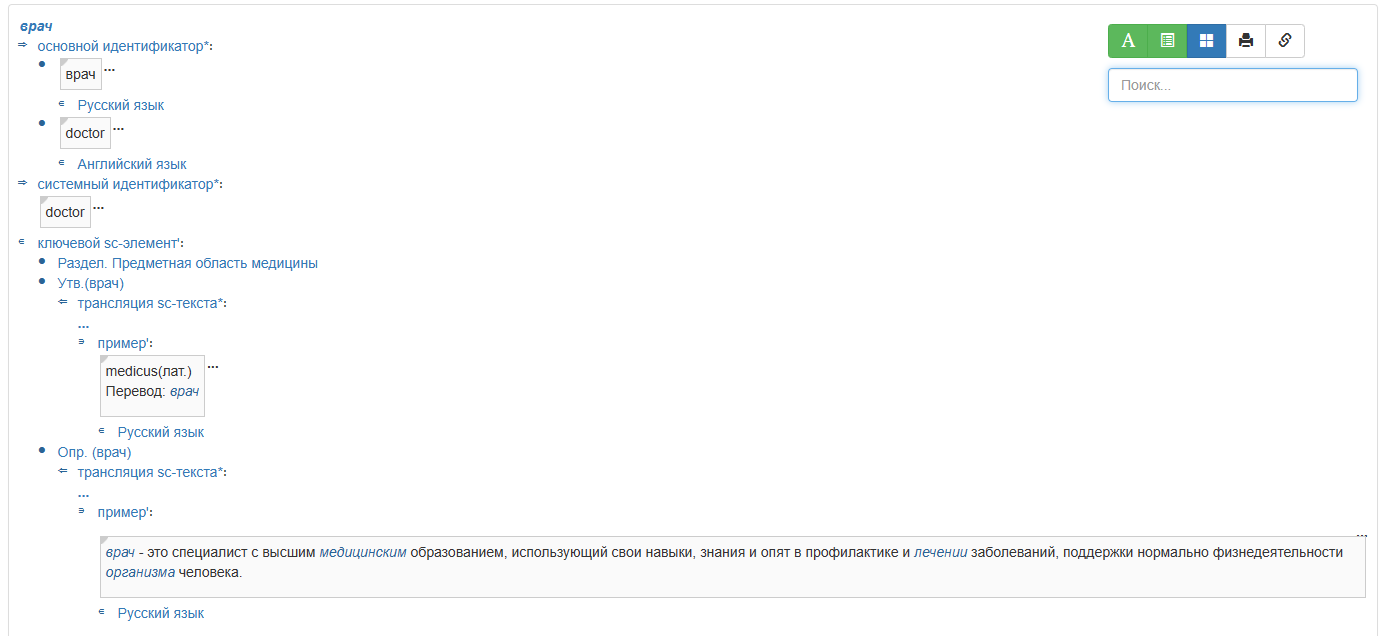
\includegraphics[width=1.0\textwidth]{sections/concept_doctor.png}
	\caption{Понятие "Доктор"}
	\label{fig:sections/concept_doctor}
\end{figure}

Фрагмент базы знаний, отображающий  понятие "Личность" \cite{bme}$,$ представлен на рисунке
~\ref{fig:sections/concept_personality}.
\begin{figure}[H]
	\centering
	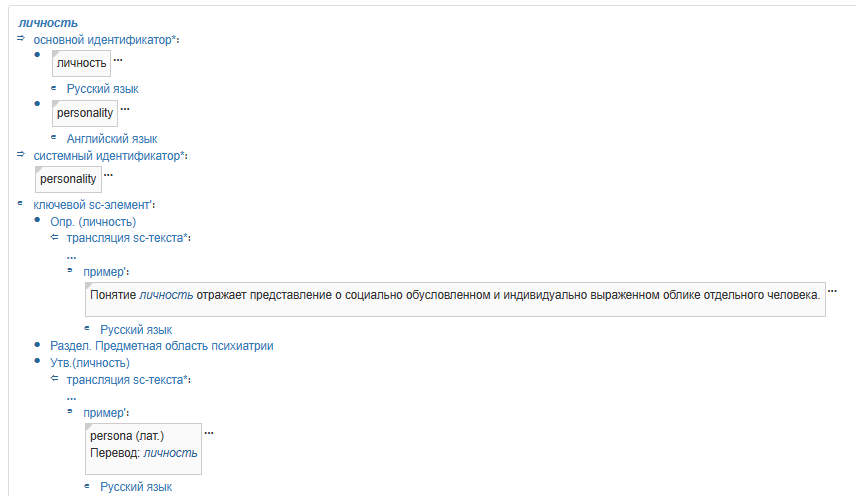
\includegraphics[width=1.0\textwidth]{sections/concept_personality.png}
	\caption{Понятие "Личность"}
	\label{fig:sections/concept_personality}
\end{figure}

Фрагмент базы знаний, отображающий  понятие "Акупунктурная точка"$,$ представлен на рисунке
~\ref{fig:sections/concept_acupoint}.
\begin{figure}[H]
	\centering
	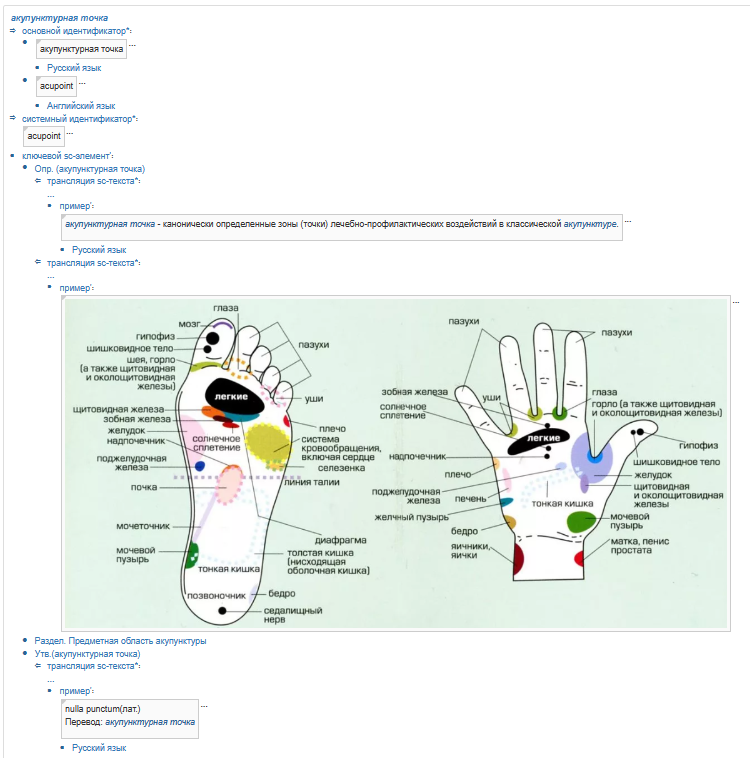
\includegraphics[width=1.0\textwidth]{sections/concept_acupoint.png}
	\caption{Понятие "Акупунктурная точка"}
	\label{fig:sections/concept_acupoint}
\end{figure}

Фрагмент базы знаний, отображающий  понятие "Игла медицинская"$,$ представлен на рисунке
~\ref{fig:sections/concept_needle}.
\begin{figure}[H]
	\centering
	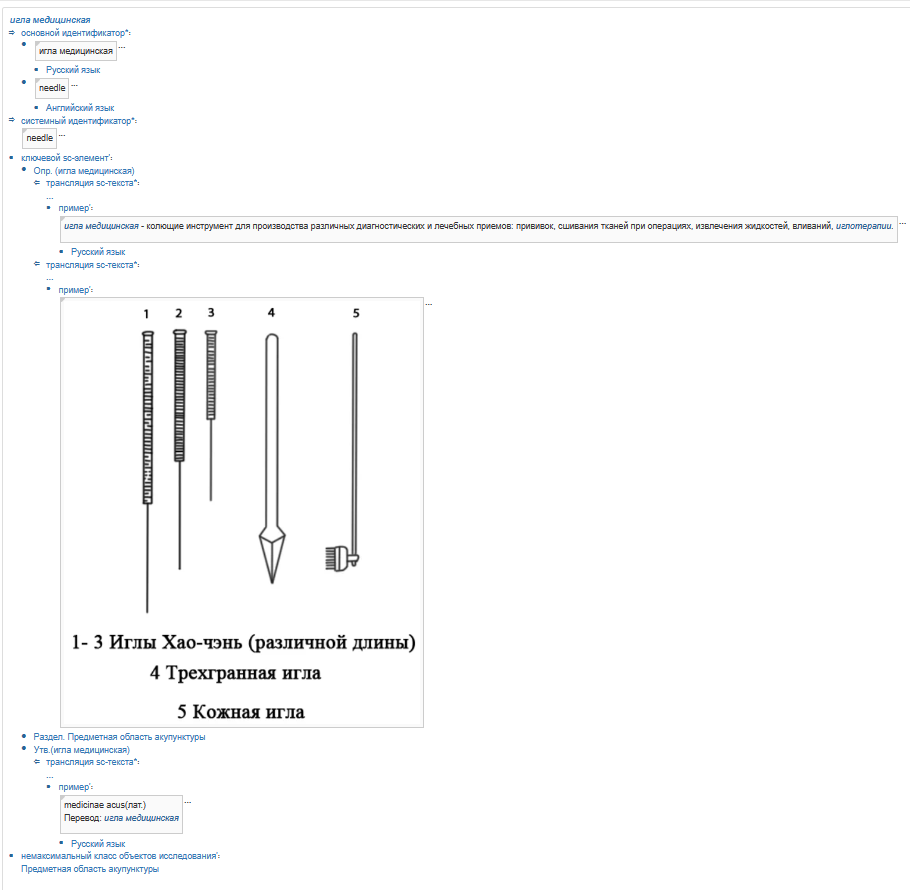
\includegraphics[width=1.0\textwidth]{sections/concept_needle.png}
	\caption{Понятие "Игла медицинская"}
	\label{fig:sections/concept_needle}
\end{figure}

Фрагмент базы знаний, отображающий понятие заболевания "Шизофрения" \cite{probolezny}$,$ представлен на рисунке
~\ref{fig:sections/schizophrenia}.
\begin{figure}[H]
	\centering
	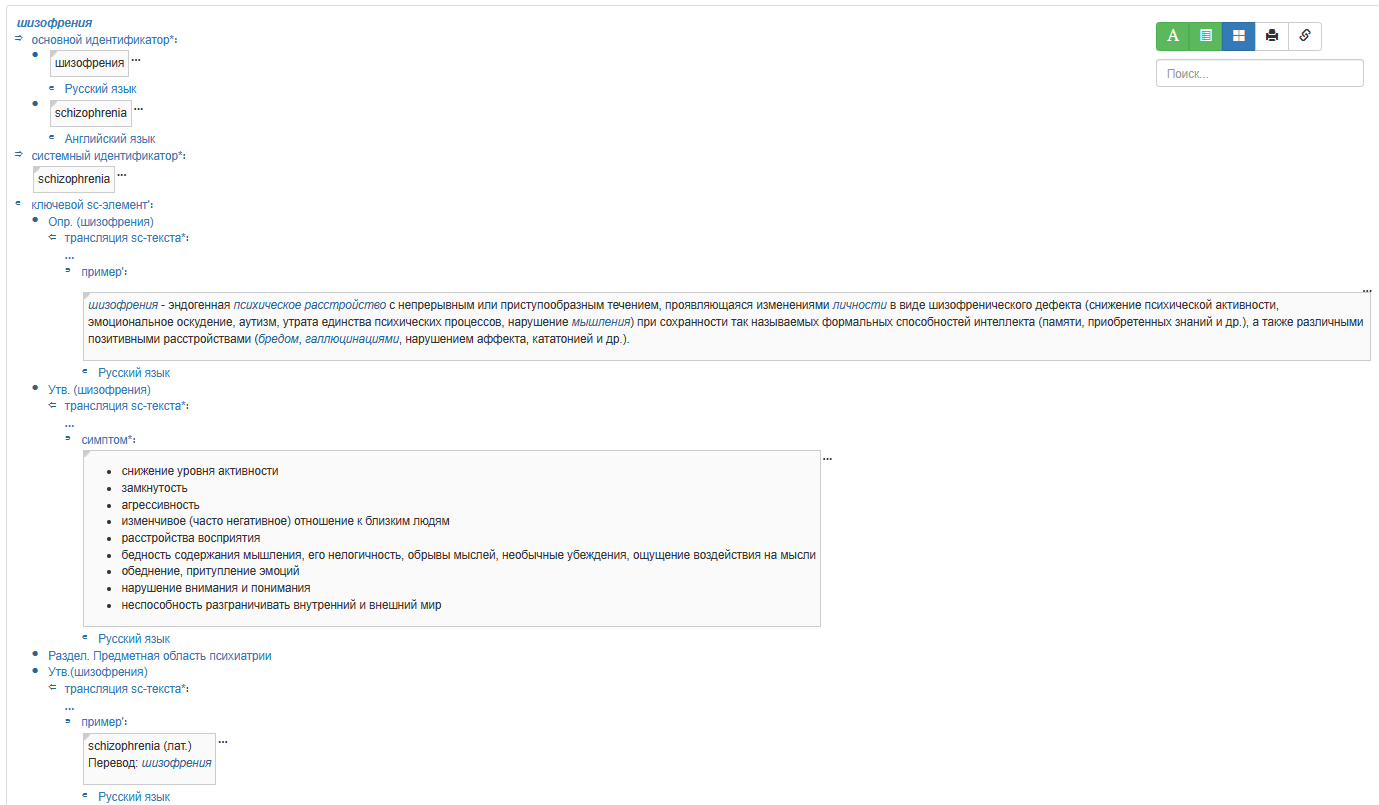
\includegraphics[width=1.05\textwidth]{sections/schizophrenia.png}
	\caption{Понятие "Шизофрения"}
	\label{fig:sections/schizophrenia}
\end{figure}

\subsection{Тестирование работоспособности базы знаний}
Тестирование базы знаний осуществляется при помощи создания шаблонов для поиска необходимых фрагментов базы знаний.
шаблон для поиска компонентов, составляющих симптомы всех заболеваний класса Шзоактивное заболевание
~\ref{fig:sections/pattern_1}.
\begin{figure}[H]
	\centering
	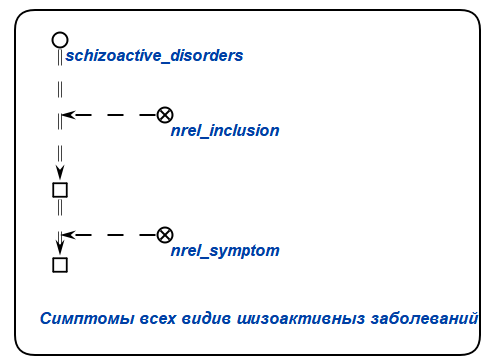
\includegraphics[width=0.6\textwidth]{sections/pattern_1.png}
	\caption{Понятие "Шаблон для поиска фрагментов базы знаний"}
	\label{fig:sections/pattern_1}
\end{figure}


Результат поиска по шаблону
~\ref{fig:sections/psy_1}.
\begin{figure}[H]
	\centering
	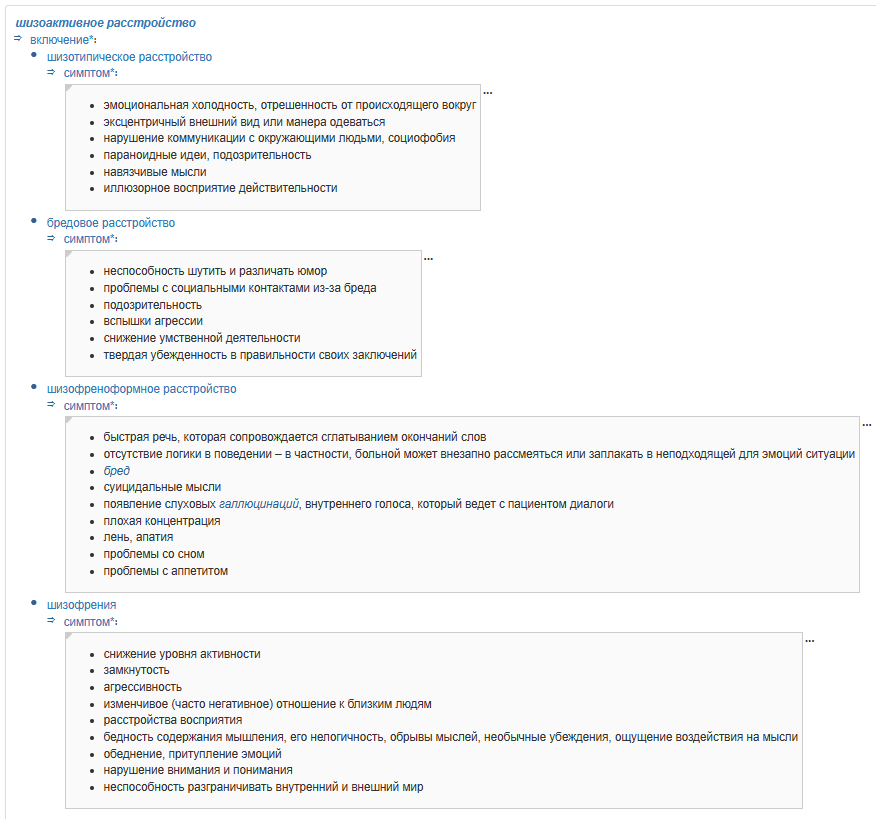
\includegraphics[width=0.85\textwidth]{sections/psy_1.png}
	\caption{Понятие "Результат поиска"}
	\label{fig:sections/psy_1}
\end{figure}

Шаблон для поиска компонентов, составляющих виды заболеваний, входящие в класс Шизоактивное заболевание
~\ref{fig:sections/pattern_2}.
\begin{figure}[H]
	\centering
	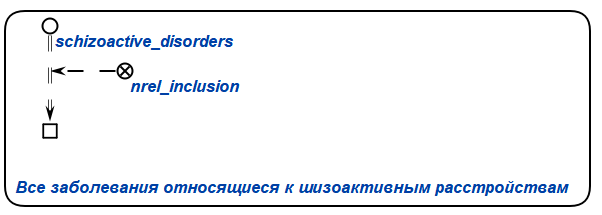
\includegraphics[width=0.8\textwidth]{sections/pattern_2.png}
	\caption{Понятие "Шаблон для поиска фрагментов базы знаний"}
	\label{fig:sections/pattern_2}
\end{figure}

Результат поиска по шаблону
~\ref{fig:sections/psy_2}.
\begin{figure}[H]
	\centering
	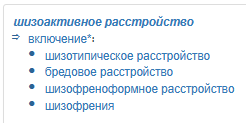
\includegraphics[width=0.5\textwidth]{sections/psy_2.png}
	\caption{Понятие "Результат поиска"}
	\label{fig:sections/psy_2}
\end{figure}


\subsection{Вывод}
Реализованная предметная область содержит большое количество необходимой и структурированной информации в области медицины, включающая в себя информацию о анатомии человека, его органов и систем органов, большое разнообразии информации о патологиях и заболеваниях, а также их симптоматику и перевод терминов на латинский язык. Особая структура данной информации делает её удобной для восприятия любым пользователем, а также быстрого и эффективного поиска необходимой информации. 

\sectioncentered*{ЗАКЛЮЧЕНИЕ}
\addcontentsline{toc}{section}{ЗАКЛЮЧЕНИЕ}

В рамках курсовой работы была разработана база знаний интеллектуальной справочной системы по медицине, включающая в себя раздел медицины,который декомпозируется на два основных раздела: традиционной и нетрадиционной медицины. Раздел нетрадиционной медицины состоит из 3 подразделов: гомеопатии, натуропатии, акупунктуры.  Раздел традиционной медицины состоит из 5 подразделов: дерматологии, психиатрии, педиатрии, офтальмологии, кардиологии. Данные разделы также делятся на свои специфические подразделы. В частности, разрабатываемая мной, предметная область медицины, традиционной и не традиционной медицины, а также предметная область психиатрии содержит подразделы: детской психиатрии, психиатрии позднего возраста, военной психиатрии и судебной психиатрии.

Суммарно в предметной области офтальмологии было формализовано более 50 абсолютных понятий. Понятия, описывающие заболеваний, содержат симптоматику, перевод на латинский язык, как и остальные(общие) медицинские термины, а также иллюстрации, которые позволяют визуализировать предоставленную информацию, что помогает лучше усвоить информацию.

Для реализации данной базы знаний использовалась технология OSTIS. Поскольку база знаний, построенная по технологии OSTIS, может описывать любой вид знаний, удобна как для машинной обработки, так и восприятия человеком. 

В результате мы положили начало созданию базы знаний интеллектуальной справочной системы по медицине.

Данная система сможет помочь студентам-медикам, медработникам и простым пользователям, интересующимся медициной, облегчить обучение и сэкономить время на поиски нужной информации. Система хорошо структурирована и наполнена большим количеством необходимой информации, что исключает необходимость использования большого количества разных источников по интересующему вопросу.

Также данная система может помочь преподавателям в медучреждениях быстро и легко находить информацию для различных проверочных  и контрольных работ для студентов. 

В дальнейшем планируется пополнение базы знаний новыми понятиями и модернизация старых. Так как в медицине существует огромное множество разделов и охватить их в рамках только лишь одной курсовой работы невозможно. Ведь медицина важнейшая область науки, которая помогает человеку улучшать своё здоровье, а также продлевать и сохранять жизнь.